\documentclass[12pt,a4paper,oneside,ngerman]{article}
\usepackage[utf8]{inputenc}
\usepackage{color}
\usepackage{tikz}
\usepackage{amsmath}
\usepackage{amssymb}
\usepackage{calc}

\title{EZS}
\author{Simon Krücken}

\begin{document}
    
%\begin{titlepage}
%    \maketitle
%\end{titlepage}
%\tableofcontents

\section[Zentrale Beschreibgrößen]{Zentrale Beschreibgrößen}

\paragraph[Defintion]{Defintion:}
Realzeitsystem haben neben Funktionalen Anforderungen auch \textcolor{red}{zeitliche} Anforderungen.

Ein Realzeitsystem besteht softwaretechnisch aus einer Reihe von Tasks und aus der System-Software.

\begin{figure}[ht]
	\centering
	\includegraphics[scale=0.5]{umlet/rt_control.png}
\end{figure}

\subsection{Technischer Prozess}
Rechenzeitanforderung = Ereignis von technischen Prozess
Releasetime = Zeitpunkt des Auftretens der RZ-Anforderung (RZ/RT = Realzeit)

\paragraph[Beispiel]{Beispiel:}
periodisches Signal \textcolor{red}{u} alle 200ms

\fbox{
	\parbox{\textwidth}
	{
		\(t_{Release,u,1}\) = 0ms \(t_{Release,u,2}\) = 200ms \linebreak
		\(t_{Release,u,3}\) = 400ms \(t_{Release,u,4}\) = 600ms \linebreak
						
		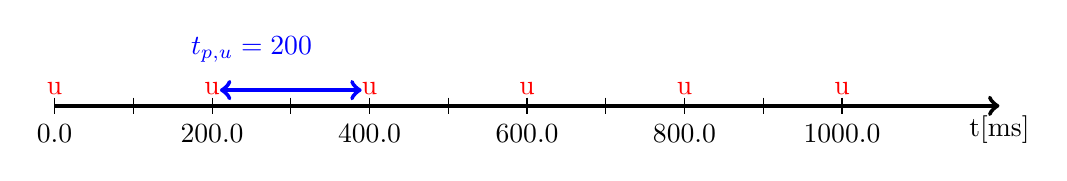
\begin{tikzpicture}
			\draw[ultra thick, ->] (0,0) -- (12,0);
			\draw[ultra thick, <->, draw=blue] (2.1,0.2) -- (3.9,0.2);
			\node[anchor=north] at (2.5,1) {\textcolor{blue}{\(t_{p,u} = 200\)}};
			\node[anchor=north] at (12,0) {t[ms]};
			\foreach \x in {0,1,2,3,4,5,6,7,8,9,10}
			\draw (\x cm,3pt) -- (\x cm,-3pt);
									
			\foreach \x in {0,2,4,6,8,10} {
				\pgfmathsetmacro\result{\x * 100}
				\draw[ultra thick] (\x,0) node[below=3pt,thick] {\result} node[above=3pt] {};
				\draw[ultra thick] (\x,0) node[above] {\textcolor{red}{u}} {};
			}
		\end{tikzpicture}
						
		\textcolor{blue}{Prozesszeit} = zeitlicher Abstand zwischen zwei \textcolor{red}{RZ-Anforderungen} gleichen Typs.
	}
}

\begin{quote}
    \(t_{Pmin,i} = minimal\) =$>$ \(t_{max,i} = \dfrac{1}{ t_{Pmin,i} }\) \\
    \(t_{Pmax,i} = maximal\) \textcolor{gray}{$<$= uninteressant}    
\end{quote}





\end{document}